\documentclass{article}
\usepackage{CJKutf8}

\title{关于收集期末复习资料的倡议}
\author{冻青铺北\\ yosunpeng@outlook.com \\ yosunpeng@gmail.com}
\date{ \today}

\usepackage{setspace}
\usepackage{indentfirst}
\setlength{\parindent}{2em}


\begin{CJK}{UTF8}{gbsn}

\usepackage{graphicx}
\graphicspath{ {./images/} }

\begin{document}
\begin{spacing}{1.5}

\maketitle
\section{Why to do that}
古语:"前人种树, 后人乘凉, 前人掘井, 后人思源." 我不管到哪里, 都常常受到别人的照顾. 无论做什么事情, 都是依靠前人做出的工作和成果. 我常思回报之心, 然而, 终究是别人给我的恩惠多, 我能回馈的少. 既然我们在做小学弟/学妹的时候, 要受到前辈的照顾, 那么当我们作为学长/学姐的时候, 能否给我们的小学弟/学妹尽心照顾呢? 我们从前辈那里受到的照顾能否回报给下一届的学弟学妹那里呢?怀着这样的心情, 我萌生了创建这个项目的念头. \\
考试, 不过一场游戏. 在规定的时间内完成规定的题目. 与其用"完成"这个中性模糊的词语, 我更倾向于用"有区别地默写"这样的短句来描述我们在考场上做的事情. 我们并不是在考场上进行知识的探索和应用, 而是在寻找考题和平时的训练题的区别, 在我们业已十分熟悉的算法模型上进行修改, 送入考试题目中的数据, 重新计算一下, 获得我们的答案. 一切都是在考场外反复模拟过的步骤和方法, 我们只是在考场上复现一下而已. 如果你们能接受我的这个假设, 那么, 考前对重点和题库的搜集整理是一件决定生死的事情, 这样的论断是很明显的. 孙子兵法曰: 庙算多者胜, 庙算少者不胜. 在考试前进行资料收集整理, 反复训练算法步骤这样的工作, 是每一届备考者都要认真辛勤劳作的事情. 我们无法把我们的大脑借给下一代, 所以我们就把资料传给他们吧, 避免这种低级而耗时的工作一代代地重复.\\
\section{Methods}
如果你同意或者部分同意我的看法, 接下来将向你说明如何参与这个有意义的项目.
\subsection{Github}
我把所有的资料上传在github. 所有的资料遵循MIT license, 这意味着一旦上传, 就放弃对资料盈利的权利. 所有的资料都是开源免费的, 可以任意下载, 修改和传播. 唯一的限制就是不能使用这些资料盈利和作商业用途. 我想这样的版权要求最符合我们创建这个项目的初衷, 也最能惠及我们的后辈们.\\
如果你是一个git的熟练使用者, 直接去fork一下我在github上的仓库, 我甚至需要你们对如何管理这个项目的建议和要求.\\
如果你和我一样都是git的新手, 我上传了\textit{Git Pro}的pdf版本, 你可以在书中找到几乎所有你所需要的知识.\\
如果你对github没有任何知识, 并且不打算在上面花费宝贵的时间, 请直接与我邮箱联系. 我会在下一小节阐述操作细节.
\subsection{Practical Problems}
如果你是git和github的使用者, 请自行解决问题. 一个GeeK做这些简单的事情还是完全没有问题的. 如果实在有, 请用邮箱联系我.\\
如果你对git和github并不感兴趣, 但是有着对我们项目的支持热忱, 并且手握重要资料, 尽管用邮箱联系我. 我将在第一时间回复你们. \\
\textbf{How to prepare your materials} \\
因为要写对资料的描述, 必然是多文件, 因此统一打包成压缩文件. zip, tar等主流压缩格式都是可以的. \\
pdf文件是首选, 所有的doc, txt类文件请先转换为pdf文件. 如果有着特殊情况, 需要保留文件的可编辑能力, 可以上传pdf和doc类两个版本的文件. 每次上传资料都要对资料进行一番描述, 讲清楚其对应的考试是哪一门课的, 哪个学院的老师在教的. 由于现在资料还比较少, 分类问题还没有困扰我们的管理者,资料分类问题将在未来确实需要得到解决时, 我们再投入精力去解决. 提交时请单独创立一个NOTE文件, pdf格式最为推荐. 请遵循以下格式: \\

\noindent 资料文件名 \\
 资料对应课程名 \footnote[1]{越详细越好, 最好有课程号, 很多课程名称相近, 弄错就麻烦大了} \\
 任课老师隶属学院名 !!!严禁!!! 禁止出现老师真名! 保持匿名是最大限度保持安全的必要举措!!! \\



如果对资料有疑问, 或者资料出现错误需要勘误, 请在该资料所在的子文件夹中的README文件中进行标注和提出正确答案. README文件是一类特殊的txt文件, 尽管像txt文件去编辑它们. 请遵循这样的格式:\\

\end{spacing}
\noindent! 错误 资料文件名  \\
 勘误者姓名\footnote[2]{我强烈建议使用昵称, 最好和社交网站所用的昵称也不一样. 保持匿名可以最大限度地保持自由和安全, 谁知道会出现什么事情. 传个资料又不会扬名立万.} + 编辑日期  \\
 错误在文件中具体位置的描述  \\
 正确的答案  \\
 你认为这样是正确的理由.\footnote[3]{当然在叙述过程会中不可避免地阐述原文出错的原因} \\
\\
\begin{spacing}{1.5}
遵循一定的格式将使README文件真正会被READ, 乱糟糟的文档没有人愿意读. \\
\textbf{How to commit your contributions}\\
Git和Github用户请自行解决.
不使用git的用户, 请先用邮箱联系我, 然后通过QQ或百度网盘传递资料给我, 剩下的事情请交给我. \\
课程文件夹已经创立的, 直接上传到对应目录下即可, 没有创立的, 联系我讲清楚课程全名, 我会解决.\\
我们项目的github网址: https://github.com/yosunpeng/postgraduate\_test\_njupt
现有的文件树图如下: \\
\begin{figure}[h]
\begin{center}
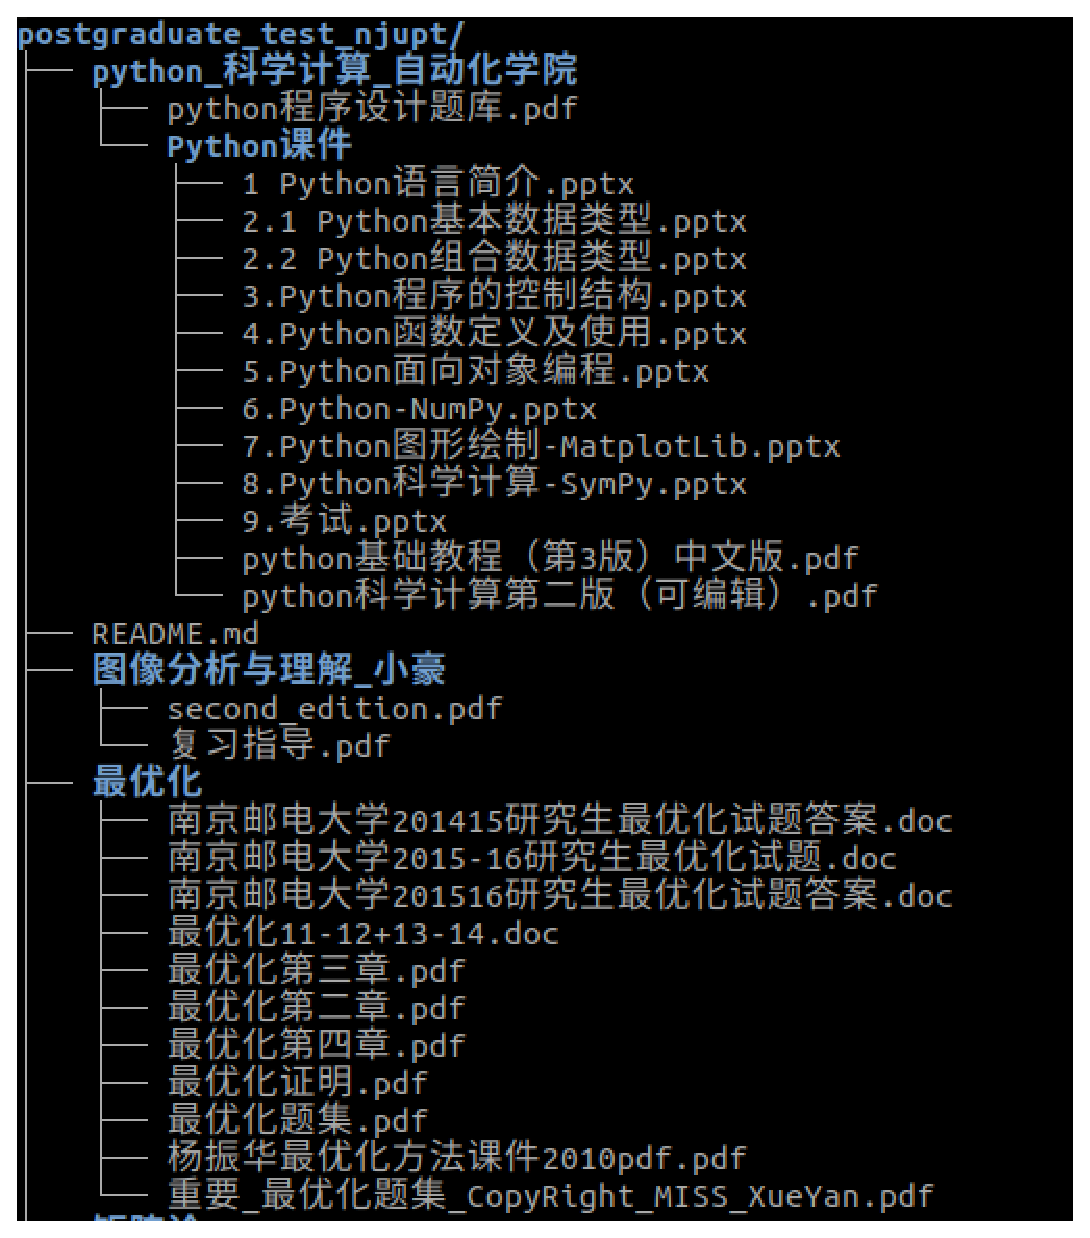
\includegraphics[scale=0.4]{1.eps}
\caption{file tree 1}
\end{center}
\end{figure}

\begin{figure}[h]
\begin{center}
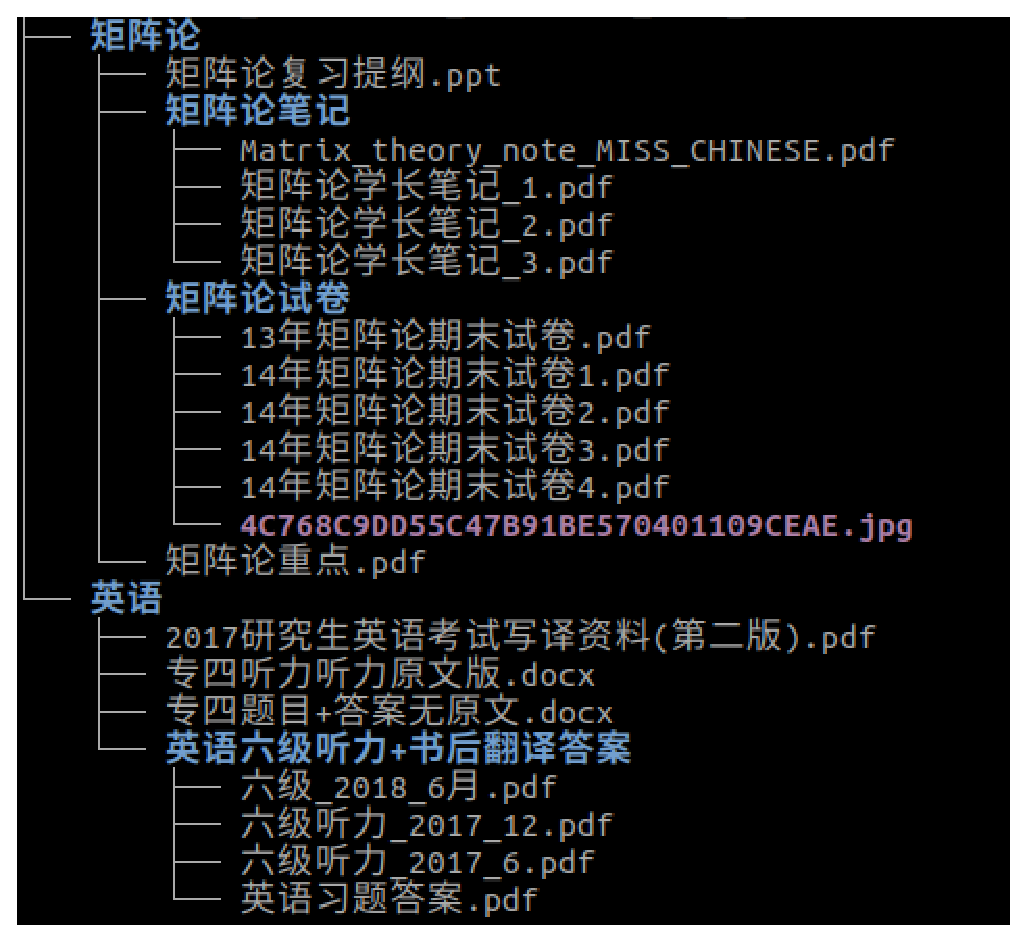
\includegraphics[scale=0.4]{2.eps}
\caption{file tree 2}
\end{center}
\end{figure}






\end{spacing}
\end{CJK}
\end{document}
